\begin{quote}
\small
\articleABSTRACT
\end{quote}



A bit of introduction here. Cite \citet{lamichhane2003}
and \citet{blades2002}.

Mention R/negenes \citep{negenes} and cite R \citep{R}.

\subsubsection{Personal history}

late to version control

\subsubsection{Reproducibility challenges}

Talk about the mess that I left myself.

\subsubsection{The R/negenes package}

Talk about maintenance and changes of the R package.


\begin{figure}

\includegraphics[viewport=133 224 464 528, width=0.55\textwidth]{../original/Nov02/R/Figs/fig1.ps}
\hfill
\includegraphics[viewport=133 224 464 528, width=0.55\textwidth]{../reproduction/Figs/fig1.ps}

\caption{Figure 1a in Lamichhane et al. (2003). Original on left. Reproduction on right.}

\end{figure}

\begin{figure}
\includegraphics[viewport=179 299 438 517, width=0.55\textwidth]{../talk/Figs/circlefig.ps}
\hfill
\includegraphics[viewport=179 299 438 517, width=0.55\textwidth]{../reproduction/Figs/circlefig.ps}

\caption{Figure 1b in Lamichhane et al. (2003). Original on left. Reproduction on right.}
\end{figure}



\begin{figure}
\includegraphics[viewport=44 245 525 508, width=0.55\textwidth]{../original/Nov02/R/Figs/fig2.ps}
\hfill
\includegraphics[viewport=44 245 525 508, width=0.55\textwidth]{../reproduction/Figs/fig2.ps}

\caption{Figure 2 in Lamichhane et al. (2003). Original on left. Reproduction on right.}
\end{figure}
